\documentclass[11pt,a4paper]{article}
\usepackage[margin=24mm]{geometry}
\usepackage[T1]{fontenc}
\usepackage{lmodern,microtype,amsmath,booktabs,array,graphicx}
\usepackage[numbers,sort&compress]{natbib}
\usepackage[hidelinks]{hyperref}
\usepackage{xurl}
\newcommand{\doi}[1]{\url{https://doi.org/#1}}
\setlength{\parindent}{0pt}
\setlength{\parskip}{5pt}
\setlength{\emergencystretch}{2em}
\renewcommand{\arraystretch}{1.15}
\newcommand{\mae}{\mathrm{MAE}}
\title{Context Controls and EEG Pairing in Retrospective Valence Prediction: An Exploratory FACED Study}
\author{Muhammad Muntazar \and Muhammad Wasif Shakeel}
\date{National University of Sciences and Technology (NUST), Islamabad, Pakistan}
\begin{document}
\maketitle
\begin{abstract}
\textbf{Purpose.} To evaluate whether tested EEG predictors improve individual retrospective valence prediction beyond available elicitation metadata on FACED, and whether their performance depends on matching EEG to the rated participant and material.
\textbf{Methods.} Seventy source and twenty development-validation participants formed three overlapping rotations of eight source and six held catalogue titles. The target was individual post-clip valence, rather than assigned emotion. Source-selected category and metadata controls were compared with spectral regression and EEGNet residual prediction. All acquisition failures remained in the scoring denominator through declared fallback. Participant/title resampling and constrained EEG swaps provided descriptive diagnostics; reserved confirmation outcomes remained sealed.
\textbf{Results.} Mean unfamiliar-title MAE was 1.2602 for the category median, 1.2156 for spectral/context regression and 1.2550 for EEGNet/context prediction on the 0--7 scale. All six corresponding rotation-level gain intervals included zero. Every pairing interval also included zero, and neural convergence remained unresolved.
\textbf{Conclusion.} These reused development panels establish neither consistent incremental EEG benefit nor equivalence to context. The study qualifies category support, preserves acquisition failures and separates predictive comparisons from pairing diagnostics. Independent confirmation and stronger baseline qualification remain necessary for broader claims.
\end{abstract}
\noindent\textbf{Keywords:} EEG; valence regression; stimulus context; FACED; participant generalization; exploratory evaluation

\section{Introduction}
EEG emotion recognition benchmarks often predict a stimulus's assigned label, whereas individual affect can differ within the same stimulus. FACED provides both elicitation categories and retrospective individual ratings \cite{chen2023faced}. Predicting an individual's valence therefore requires distinguishing useful EEG information from information already supplied by the experiment.

This distinction is established prior work. Gerster et al. investigate FACED stimulus confounding \cite{gerster2026stimulus}; their later released code includes individual categorical targets, clip-held evaluation and nested tuning \cite{gerster2026code}. The June preprint and August code revision have not been authenticated as identical versions. Kong et al. examine video/time priors and physiological residuals on familiar videos \cite{kong2026priors}, while Wang et al. separate shared and individual continuous affect trajectories \cite{wang2026shared}. Accordingly, we claim neither the first context control nor a new neural architecture.

Our question is narrower: for individual retrospective FACED valence, do tested predictors improve over supplied metadata on new people and held catalogue titles? We contribute a reproducible exploratory evaluation that qualifies baseline selection against category support, retains acquisition failures, and checks participant/material pairing. EEGNet is an established compact baseline \cite{lawhern2018eegnet}. Other established EEG representations exist \cite{zhang2023spatiotemporal}; the present bounded search does not qualify an optimal EEG decoder.

\section{Methods}
\subsection{Population, target and development panels}
FACED's item-10 post-clip valence, with negative-to-positive anchors on 0--7, is the outcome. Endpoints and midpoint ratings are retained without thresholding. Metadata exclusions and participant/material reservations preceded rating decoding. Neutral clips 13--16, sharing the title \emph{Blue}, are outside the specified non-neutral elicitation population; clip 22 is excluded because version-dependent marker duration and footage correspondence remain unresolved. This is not an evaluation of all FACED materials.

The reservation contains 70 source, 20 development-validation and 33 protected participants. Fourteen catalogue-title families enter development; eight other families remain reserved. Three rotations use eight source titles and six unfamiliar titles, each with one clip. Each rotation has 560 source trials and 120 unfamiliar-title validation trials; a familiar-title arm adds 160 trials from the same validation people. Exact identities and splits are released. Source and validation people are disjoint; rotations share people and materials.

\emph{Unfamiliar} means absent from the rotation's source-title catalogue. It does not measure personal familiarity or prove distinct physical footage. Original media bytes and playback latency remain unauthenticated. The unfamiliar arm has no Fear or Inspiration titles. Every source rotation has one title for each of eight categories, confounding source category with title. Inference is conditional on the category metadata being supplied.

\subsection{EEG processing and availability}
Qualified headers calibrate signed ADC counts into microvolts at native 250/1,000 Hz. A trial-local 32-second interval ending at the recorded end marker undergoes common-average referencing, a 50-Hz notch, 0.5--45-Hz forward/backward Butterworth filtering and polyphase resampling to 128 Hz. Edge trimming leaves a 28-second core: seven nonoverlapping four-second windows on thirty scalp channels. This late interval predicts whole-clip retrospective valence, not momentary emotion; processing is offline and acausal.

Fixed amplitude rules permit spherical-spline repair of at most three channels \cite{perrin1989spherical}. Eight of 980 unique source trials require repair; all source trials pass the final availability policy. Raw rail occupancy, stuck counts, processed amplitude, line power and numerical validity determine availability independently of an evaluated rating. Fifteen of 280 validation trials have unavailable EEG, including fourteen for one participant. All trials and participants remain scored. EEG-only models use a source global-median fallback; historical joint models use their declared source-fitted full-context fallback. Thresholds and operator details are provided in the supplement. The policy follows earlier development inspection and is part of the adaptive programme.

\subsection{Controls, selection and diagnostic contrasts}
Context comprises eight assigned-category indicators, three acquisition-group indicators, catalogue duration and presentation ordinal. These are supplied study metadata, not the evaluated participant's rating; unfamiliar-title identity and held-title rating consensus are unavailable. Spectral EEG contributes 150 log-band-power features from five bands averaged over seven windows. Covariance/kernel alternatives and all fifteen historical conditions are retained in Supplementary Table S1.

A baseline-selection diagnosis found that jointly withholding source people and titles removed the held titles' categories. The category prior then reverted to a global median. That diagnostic therefore measured a different information condition from the category-known validation task. We qualified five candidates using five person-held source folds that retain every category: global, coarse-valence and category medians, category-only Ridge and full-context Ridge. Each transform uses its fold's source rows; Ridge alpha is selected from \(\{0.1,1,10,100,1000\}\). This procedure evaluates new people on source titles, not new-title generalization. Category median is selected in every rotation, and both Ridge families select alpha 0.1. No validation result chooses among these revised controls.

The spectral/context anchor retains historical joint Ridge alpha 100. EEGNet-8,2 uses a local scalar head and two-seed ensemble, trained with one loss per original trial after averaging window outputs. Its context-residual variant learns against person-excluded source context offsets and uses the full source context fit at inference. Twenty fixed neural fits run 120 epochs. Schedules are selected on rotation-0 unfamiliar validation and transferred to rotations 1/2. These anchors were developed using earlier outcomes; their comparison with newly qualified controls is exploratory.

A separately declared retrospective sensitivity uses cached full-context Ridge predictions at the same alpha 100 as spectral joint Ridge, with identical source rows and source-only scaling. On unavailable EEG, both receive the historical joint model's original fallback. Thus failure cases contribute zero incremental gain. Available predictions and joint predictions are unchanged; no models are refitted. This matched contrast tests adding spectral features within the fixed regression recipe; it does not identify cerebral or emotion-specific information.

Two constrained swaps retain recipient metadata and outcome: another validation person's EEG from the same title/acquisition group, or the same person's EEG from another title within coarse valence. Within eligible non-singleton strata, thirty-two fixed derangements exclude self-donors. Eligible donors must have available EEG; singleton strata remain unperturbed. For EEGNet, cached raw residual corrections move while the recipient's context offset remains fixed. Repeat losses, rather than predictions, are averaged before aggregation. Unavailable recipients retain fallback.

\subsection{Endpoints, uncertainty and audit}
Predictions are clipped to 0--7. MAE equally weights people and title families, averaging clip absolute errors within a cell; here it equals trial MAE. Incremental gain is comparator MAE minus joint-model MAE. Swap sensitivity is swapped minus original MAE. We report all rotations separately; their mean summarizes dependent panels.

Paired crossed participant/title bootstrap intervals use 4,000 draws. They are descriptive percentile intervals on reused development data, not selection-adjusted confidence guarantees, equivalence tests or causal effects. Six held titles limit precision; more people cannot remove uncertainty from limited materials \cite{westfall2014power}. Crossed resampling follows the general rationale of multi-factor bootstrap methods \cite{owen2007,owen2012}.

Centered two-way additive sums of squares describe participant, title and residual rating variation. A single rating per cell cannot separate interaction, measurement error or reliability. Public identity, prediction and interval audits pass. A separate source checkpoint/window check covers 24 fixture/seed forwards and 48 offset comparisons; validation swaps reuse authenticated cached corrections, without a new independent waveform-forward replay. Reserved outcomes are not accessed.

\section{Results}
\begin{table}[tbp]
\centering
\small
\caption{Unfamiliar-film validation MAE on the original 0--7 rating scale (lower is better).}
\label{tab:primary}
\begin{tabular}{lrrrr}
\toprule
Predictor & R0 & R1 & R2 & Mean \\
\midrule
Category median (source selected) & 1.222 & 1.232 & 1.327 & 1.260 \\
Category Ridge (source selected) & 1.252 & 1.234 & 1.315 & 1.267 \\
Full-context Ridge (source selected) & 1.253 & 1.220 & 1.338 & 1.270 \\
Matched context, $\alpha=100$ (sensitivity) & 1.258 & 1.210 & 1.311 & 1.260 \\
Spectral + context Ridge (frozen) & 1.259 & 1.177 & 1.211 & 1.216 \\
EEGNet + context residual (frozen) & 1.191 & 1.311 & 1.263 & 1.255 \\
\bottomrule
\end{tabular}
\par\medskip\begin{minipage}{0.97\linewidth}\footnotesize Each panel contains 20 held people and six title families; all outcomes, including unavailable EEG, are retained. The mean is a descriptive average of dependent rotations. Category/full-context selection is source-person-only and familiar-title CV; frozen EEG recipes were previously development selected. Matched context is a separately declared retrospective sensitivity with the historical joint fallback shared by both methods on acquisition failures.\end{minipage}
\end{table}


Category median MAE averages 1.2602 (Table~\ref{tab:primary}). Relative spectral/context gains are \(-0.0368\), \(+0.0549\) and \(+0.1158\), averaging 0.0446. EEGNet/context gains are \(+0.0314\), \(-0.0794\) and \(+0.0636\), averaging 0.0052. All six unfamiliar-title gain intervals include zero. These whole-recipe comparisons use the source-selected category control. Fixed-alpha matched-context gains are \(-0.0006\), \(+0.0332\) and \(+0.0995\), averaging 0.0440; all three intervals also include zero (Supplementary Table S3). The historical per-panel minimum of five context models remains a labelled retrospective envelope, not a deployable selected control.

Familiar-title mean MAE is 1.1723 for category median, 1.2094 for spectral/context and 1.2918 for EEGNet/context. EEGNet's rotation-2 familiar gain is \(-0.1852\), with descriptive interval \([-0.3498,-0.0143]\); this adverse result is retained. Other familiar contrasts include zero. Five of six selected neural trajectories continue improving source MSE by more than 10\% between epochs 60 and 120. Source learning therefore does not establish converged validation performance or adequate model optimization.

\begin{table}[tbp]
\centering
\small
\caption{Descriptive additive squared-deviation components of retrospective valence.}
\label{tab:variation}
\begin{tabular}{lrrrrr}
\toprule
Role & People & Titles & Person & Title & Residual \\
\midrule
Source & 70 & 14 & 9.95\% & 43.29\% & 46.76\% \\
Validation & 20 & 14 & 12.83\% & 42.31\% & 44.86\% \\
\bottomrule
\end{tabular}
\par\medskip\begin{minipage}{0.97\linewidth}\footnotesize Complete person-by-title rectangles contain one rating per cell. The residual includes person--title interaction and unexplained variation; these fractions do not identify measurement noise, response style, reliability or a prediction floor.\end{minipage}
\end{table}


Title terms account for approximately 43.3\% of source and 42.3\% of validation squared deviations (Table~\ref{tab:variation}). Participant terms account for 10.0\% and 12.8\%. These summaries motivate context comparison without attributing the residual to decodable EEG.

\begin{figure}[t]
\centering
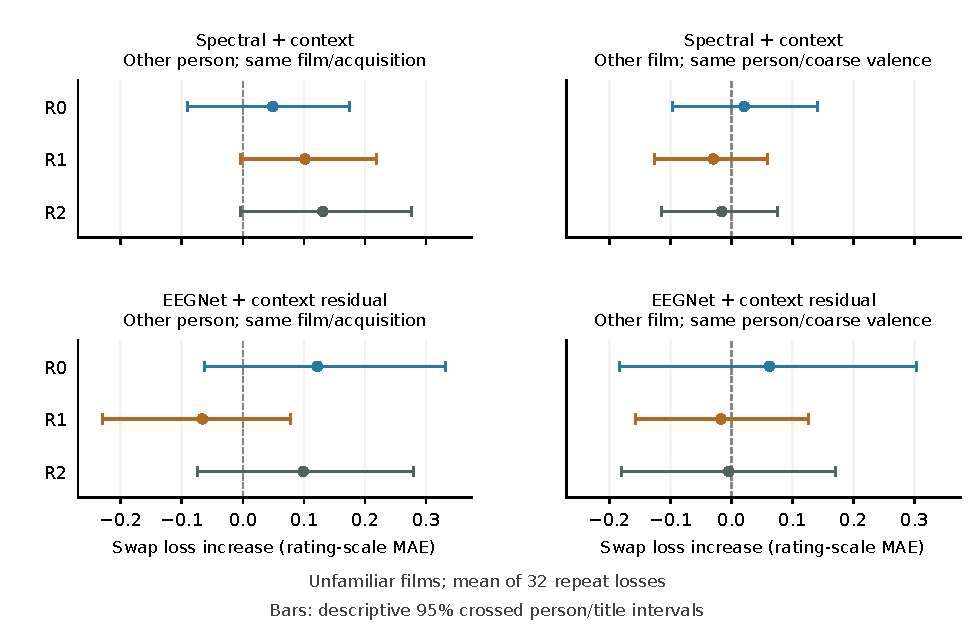
\includegraphics[width=\linewidth]{figures/pairing_publication.pdf}
\caption{Unfamiliar-title pairing diagnostics. Positive change means swapping raises loss. Points average 32 repeat losses; bars are descriptive crossed participant/title intervals. Same-title/person swaps constrain different factors; ineligible and unavailable recipients remain unchanged. All twelve displayed intervals include zero. Supplementary Table S4 retains all twenty-four panels, including familiar materials.}
\label{fig:pairing}
\end{figure}

Same-title/acquisition person swaps increase spectral-model unfamiliar MAE by 0.0487, 0.1017 and 0.1309; neural changes are 0.1221, \(-0.0665\) and 0.0987 (Fig.~\ref{fig:pairing}). Same-person film swaps yield smaller, mixed changes. All twenty-four pairing intervals include zero. Eligible unfamiliar recipients number 108/107/107 for person swaps and 114/113/113 for film swaps, from 120 per rotation. The remaining recipients stay in every score.

\section{Discussion}
The study-specific baseline audit identified an information mismatch: withholding the only source title for a category also removes that category's support. Category-preserving source selection is appropriate for the supplied-category condition, but cannot certify transfer to unfamiliar titles. It selects a competitive simple comparator, making model utility easier to assess without selecting a reference from validation outcomes.

Spectral/context prediction has a small favorable mean gain against that comparator, but the direction varies and every unfamiliar interval includes zero. Neural benefit is less consistent and optimization remains bounded. Neither result demonstrates equivalence, absence of affective EEG information, or superiority to existing state-of-the-art methods. Pairing tests diagnose dependence within constrained donor pools; acquisition, artifacts and person characteristics can contribute. They do not isolate a causal emotional mechanism.

Limits include a single corpus, one retrospective rating per cell, late-interval EEG, few held titles, category/title confounding, unavailable media authentication and supplied metadata that may not exist in deployment. Acquisition fallback preserves operational denominators but changes the effective model. Adaptive model exploration, reused validation outcomes and overlapping rotations preclude confirmatory inference. Stronger baselines, independently fixed selection and a suitable second public corpus would strengthen external validity. A separately preserved confirmation protocol remains inactive; no protected result supports this paper.

\section{Conclusion}
This exploratory FACED study makes baseline information, acquisition fallback and pairing constraints explicit. Context-only category prediction is competitive with the tested EEG recipes; consistent incremental EEG benefit remains unestablished. The released diagnostics support a bounded evaluation case study, rather than a novel architecture or a general negative conclusion about EEG emotion recognition.

\section*{Declarations}
This secondary analysis collected no new participant recordings. FACED's source publication reports its original ethics and consent procedures \cite{chen2023faced}; source-study approval does not constitute a new institutional exemption. Anonymous development predictions, evaluation code and audit receipts are available at \url{https://github.com/Overproness/GRU-XNet_EEG_Emotion_Recognition}; original recordings and rating archives are not redistributed. Generative-AI assistance supported manuscript drafting, code preparation and checking; the authors remain responsible for the work.

\bibliographystyle{unsrtnat}
\begingroup
\small
\setlength{\bibsep}{3pt}
\bibliography{references}
\endgroup
\end{document}
